\section{Packets Type Overview ("`EOFpkg"')}
\label{eofpkg}
Based on the previous definition of data types and messages, one
can distinguish between the following packet types:
\begin{itemize}
\item Messages: (internal) plaintext packets (\ref{eofmsg}, p. \pageref{eofmsg})
\item Onions: multiply encrypted packets (\ref{eofonion}, p. \pageref{eofonion})
\item Postcards: packets containing transport protocol dependent header (\ref{eofpostcard}, p. \pageref{eofpostcard})
\end{itemize}
Messages are the innermost packet type and can only be seen within
the implementation.
Messages are then bundled into a multi layer onion. 
Each layer contains messages after decryption.
Onions are put onto a \textit{postcard packet} 
afterwards and are sent out on the network.
Figure \ref{packettypes} visualises the differences between the 
different packet types.
\begin{figure}[htb]
    \centering
    \caption{Packet Types}
    \label{packettypes}
    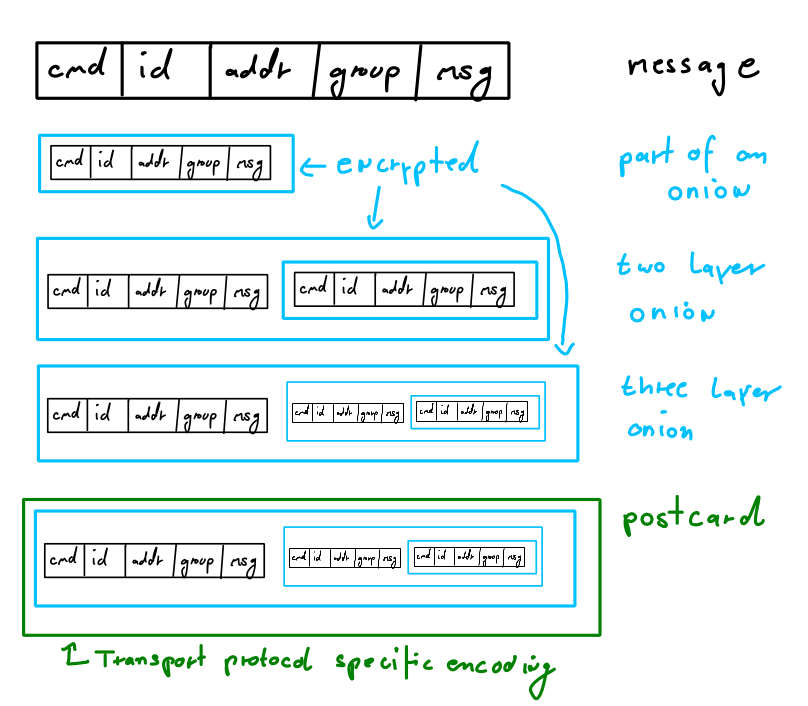
\includegraphics[scale=0.7]{packet-types.png}
\end{figure}
